\documentclass[oneside,a4paper,english,links]{amca}
%
\usepackage{graphicx}
\usepackage{amsmath,amsfonts}

\title{REAL TIME DIRECT VOLUME RENDERING OF BREAD CRUMBS}

\author[a]{Rodrigo Baravalle}
\author[b]{Leonardo Scandolo}
\author[c]{Claudio Delrieux}
\author[d]{Cristian G. Bauza}
\author[a]{Juan C. G\'omez}
%
\affil[a]{Laboratory for System Dynamics and Signal Processing, FCEIA, Universidad Nacional de Rosario, CIFASIS-CONICET,
Ocampo y Esmeralda, S2000EZP~Rosario, Argentina,
baravalle@cifasis-conicet.gov.ar, \url{http://www.cifasis-conicet.gov.ar/grupo4.html}}
%
\affil[b]{Computer Science Department, FCEIA, Universidad Nacional de Rosario,
Pellegrini 2050, 2000~Rosario, Argentina,
leonardo@fceia.unr.edu.ar, \url{http://web.fceia.unr.edu.ar/es/institucional/escuelas/118-departamento-ciencias-de-la-computacion-ecen.html}}

\affil[c]{Department of Electrical Engineering and Computers, Universidad Nacional del Sur - IIIE-CONICET,
Avenida Col\'on 80, 8000FTN~Bah\'ia Blanca, Argentina,
cad@uns.edu.ar, \url{http://www.ingelec.uns.edu.ar/}}

\affil[d]{Instituto de Investigaci\'on PLADEMA-Facultad de Ciencias Exactas - UNICEN,
Campus Universitario, Paraje Arroyo Seco, (B7001BBO) Tandil, Buenos Aires, Argentina
crgarcia@exa.unicen.edu.ar, \url{http://www.exa.unicen.edu.ar/es/d\_investigacion/inst\_pladema/index.html}}


%% NOTE: IF ALL AUTHORS BELONG TO THE SAME AFFILIATION
%% USE THE `\voidaffil' MACRO FOR THE AFFILIATION CODE.
%% Example:
%% \author[\voidaffil]{First A. Author}
%% \author[\voidaffil]{Second B. Author}
%% \author[\voidaffil]{Third C. Author}
%% \author[\voidaffil]{Fourth D. Author}
%% %
%% \affil[\voidaffil]{Grupo de Mec\'anica Computacional,
%% Universidad Nacional de Villa Carolina,
%% Los Alerces 3492, 4200 Villa Carolina, Argentina,
%% gmc@uncarolina.edu.ar, http://www.uncarolina.edu.ar/gmc}

\begin{document}
\vspace{3cm}

\maketitle

%% To set PDF METADATA: uncomment and replace fields in
%% UPPERCASE with appropriate values. 
%% 
%% \hypersetup{
%%   pdfauthor={AUTHORS},
%%   pdfkeywords={KEYWORDS},
%%   pdftitle={TITLE}
%% }
%%
%% For instance
%% \hypersetup{
%%   pdfauthor={Sponge B. and Star P.},
%%   pdfkeywords={multiphase flow, air-liquid mixtures},
%%   pdftitle={A new model for multi-phase flow}
%% }
%%
%% NOTE: To set the metadata is recommended but not absolutely
%% neccesary. 
%% This was done before with the \pdfinfo command,
%% but according to this post:
%% http://de.nntp2http.com/comp/text/tex/2008/12/5358fd061de9703a781885a5dcf98364.html
%% if `hyperref' is used, then you must use \hypersetup{} not \pdfinfo{}

\begin{keywords}
Direct Volume Rendering, Bread Crumb, Real Time.
\end{keywords}

\begin{abstract}
Photo-realistic modelling and rendering of materials with complex internal structure poses a hard challenge in the Computer Graphics community. In particular, bread crumbs consist of a complex translucent material with a porous structure that presents different details at different scales. In realistic bread crumb rendering there are several light phenomena involved such as subsurface scattering, self-shadowing, self-occlusion, reflectance, and absorption. Current approaches to recreating these phenomena using a realistic approximation to the rendering equation, i.e., accounting for global illumination as in ray and path tracing, are computationally expensive and generally require a detailed mesh of the bread crumb.

Current solutions set up a complex capture procedure, in which the light reflecting off the material is sampled at different angles. That information is used to reconstruct a material model. While this solution accounts for several desired properties of this material, it presents several drawbacks which difficults its practical applications: high computational costs, the requirement of complex capture procedures, and poor image variability.

In this work, we propose the study and implementation of a GPU based direct volume rendering on a scalar field representing the internal structure of a bread crumb without requiring any intermediate steps. The images obtained show promising results at interactive and real time frame rates. The crumb is represented as a 3D scalar field, which is computed in two steps. The first uses a particle system based generation procedure, and the second uses dynamic systems to evolve the particles mimicking the bread making process.
\end{abstract}

\section{INTRODUCTION}

The appearance of bread crumbs and other baked materials, such as pizzas and cookies, has been considered a challenge to render due to the complex interaction of light outside an inside the material. Computational costs (memory storage and cpu time) of these physical simulations made its rendering impractical in areas in which interaction with the final user is critical. The exponential growth in computing power, based on the massive parallel design of modern graphics cards \citep{Yeo09,Harris06}, has made possible to simulate some light phenomena at acceptable computational rates, but the field is still a subject of research \citep{Voglsam2013}.

The geometry of these materials are the result of complex mechanisms which involves physical deformations and chemical reactions. For instance, in bread making, two different processes are involved: proofing and baking. Proofing involves chemical reactions between the living yeast and the dough. The yeast produces $CO_{2}$ which in turn makes bubbles in dough \citep{Shah1998}. In the baking process \citep{Mondal2008}, temperature changes these shapes in several ways \citep{Scanlon2001}, giving bread its final internal structure. A few attempts to synthesise a model of this geometry has been made \citep{VanDyck2014,Anyone}, but the structure obtained is the result of an artistic design, and, in the case of x-ray tomography, the variability of the structure is limited to the amount of captures made. In this work we propose to employ dynamical systems \citep{Strogatz2001} in order to evolve particle systems \citep{Reeves83} that we have previously designed \citep{Baravalle2011}, trying to mimic the bread making process (proofing and baking). Many complex processes as weather and fluids are governed by differential equations which describes their dynamics and appearance. This idea is employed in this paper for describing the bubble growth process in bread. This process outputs a structure which is perceived as if bubbles were growing in a fluid, similar to patterns found in bread crumbs.

The mechanism for rendering these internal structures depends largely on the data structure chosen for representing them. If a mesh of triangles is used, it should be computed from initial data. Nevertheless such process could be a non-trivial task due to the porous structure of bread, and is potentially high memory demanding. Trying to represent the material as a surface is not adequate since the material presents visible structures on its surface. Bread is classified as a non (or quasi) homogeneous \citep{Tong2005}, due to the presence of mesostructures (bubbles) on it. In other words, typical solutions as Bidirectional Reflectance Distribution Functions (BRDF) \citep{Kurt2009} and Bidirectional Surface Scattering Reflectance Distribution Functions (BSSRDF) \citep{Donner2009} are not completely adequate since mesostructures cannot be addressed with these methods. A material model is defined in \citep{Tong2005} which solves these limitations. It is true that this method shows good results, but the main drawbacks of this approach (complex capture procedure involved, computational costs, poor image and structure variability), made it difficult for a wider application.

In this paper we propose to apply Direct Volume Rendering (DVR) \citep{Levoy1988,Kruger2003} to a scalar field in order to render the bread crumb structure. DVR applies ray marching through the volume in order to accumulate different properties for each pixel. The method does not use intermediate structures, simplifying the modelling process. In addition, the shape of the bread crumb can be defined in real time on the GPU, making it possible to make arbitrary cuts, slices and deformations of the 3D structure in real time. Also, the crust of the bread can be easily defined by artists along with its own properties like colour and translucency. Results show promising results at real time rates. 

This paper is organised as follows. In section 2 the theory of dynamic systems and DVR is introduced. In section 3 the results obtained in the 3D structure generation and rendering are shown and discussed. In section 4 the conclusions are summarised, as well as possible future works.

\section{MATERIALS AND METHODS}

\subsection{Particle Systems}

Early approaches in computer graphics tried to represent nature employing euclidean geometry, in other words, combining point, lines, surfaces, spheres, cylinders, cubes, etc. Nevertheless, nature is complex to describe in terms of this geometry. The shape observed in mountains, coastlines,  and almost every natural object presents irregularities which are difficult or impossible to represent using this approach. Other geometries such as fractal geometry \citep{Mandelbrot83} emerged and claimed to describe natural phenomena more adequately. With this new perspective, previous phenomena could be better modelled and rendered. 

At the same time, several techniques for non euclidean objects emerged. Particle Systems \citep{Reeves83} were designed for representing phenomena which has no well defined surface, like water, smoke and fire. These systems are composed of entities called {\em particles} which evolve its properties in time. As an example, in rendering fireworks, each particle begins its trajectory in a common space position, and each time step its position changes following a parabola. Different particles follow different parabolas. An image is obtained each step and an animation can be seen. For obtaining other effects such as fire, properties as colour, size and direction can be modified depending on time. Particles can also affect each other.

In a previous work \citep{Baravalle2011}, we employed Particle Systems for texture synthesis. Each particle had an initial random position in the image, and evolves trying to avoid other particles, similar to the concept of cellular automata on a plane. Promising results were obtained for wood and painting textures. The growth functions used were mainly random growth, vertical, horizontal and diagonal. In this work, we propose to extend it to space, and use a system of differential equations to control the growth of the self-avoiding particles to mimic the bread making process. Next section establishes the system employed to evolve the particles in time.

\subsection{Dynamical Systems}

The subject known as Dynamics deals with {\em change} \citep{Strogatz2001}. The study on Dynamics began in previous centuries with Isaac Newton's studies. Among his contributions, Differential Equations can be found. These equations deals with the difficulty (or impossibility) of finding analytical equations for these dynamical processes. After a model describing the problem is defined, the differential equations obtained are simulated and approximate solutions are derived for each step of the simulation. Dynamical Systems are concerned about processes that evolve in time, as economics, heat transfer, and fluids. With the development of computers in the last century, the field has been able to obtain insight in areas which were impossible before, since the calculations were too difficult to be performed by humans, for instance, Fractals \citep{Mandelbrot83} and Chaos.

To solve dynamical systems, numerical approximations are used. Its computational costs change depending on the complexity of the problem and the number of equations involved. We propose to employ a subfield of differential equations, named Ordinary Differential Equations (ODE) for the purposes of this work. In ODEs, time is treated as the only variable, and the equations show the relationship between the derivatives of the variable and the variable itself. 

Generally speaking, ODEs can be represented by the following set of equations:
\begin{equation} \label{eq:simple}  
\begin{aligned}
\dot{x_{1}} = f_{1}(x_{1},\ldots,x_{n}),\\
\ldots\\
\dot{x_{n}} = f_{n}(x_{1},\ldots,x_{n}),
\end{aligned}
\end{equation}

where $\dot{x_{i}}$ represents the derivative of $x_{i}$ with respect to the variable $t$. The variables $x_{i}$ and the functions $f_{i}$ are defined for each problem. In this work, each variable represents a Cartesian coordinate in space, {\em i.e.,} $x_{1}$ is $x$, $x_{2}$ is $y$ and $x_{3}$ is $z$ and the set of $f_{i}$ will be defined in order to capture the bread crumb structure.


\subsection{Direct Volume Rendering (DVR)}

The technique of direct volume rendering attempts to provide a
2-dimensional representation of a volume defined by a discreet
3-dimensional density function. Rays are casted from the point of view
of a camera in a virtual scene and the density function is used to
compute the amount of light that the camera receives from the
direction of that ray. This is done by sampling the density function
along the ray in order to approximate the effect different light
phenomena such as extinction, transmittance and scattering among
others. The light information gathered from these rays are then used
to compute the color of the pixels in the final image.

Radiance is the amount of light that passes, or is emitted, from a
point and falls within a given solid angle. When inspecting the amount
of light received for a given ray, what we are really doing is
approximating the radiance from a distant point along the direction of
the ray. The radiance value is approximated by: 

\begin{equation} \label{eq:general_radiance}  
L(p_n) = L_b + \int_{p_0}^{p_n} \frac{\partial I(t)}{\partial p} \, dt.
\end{equation}

Where $L_b$ is the background radiance, $p_0$ and $p_n$ are the
closest and furthest visible points along the ray direction,
respectively, $L(t)$ is the radiance sampled at point $t$, and
$\partial p$ is the distance between sampled points. For the purposes
of computing $L(p_n)$, the integral is approximated by a sum.

Exctinction is the loss of photons in a ray shaft due to absorption in
the participating media and scattering to other directions. Some of
the photons from the shaft will collide with the particules in the
surrounding media and be absorbed and transformed to energy, mostly
heat. Others will bounce and move along other directions. This is
approximated using an absorption coefficient for the media, $k_a$ and
a scattering coefficient $k_s$. If the scattering effect is neglected,
the formula for radiance after absorption over a distance $\partial p$
is:

\begin{equation} \label{eq:absorption_radiance}  
\begin{aligned}
\frac{\partial I(t)}{\partial p} = -k_a L(p). 
\\
\\
L(p_n) = L_b \ e^{-\int_{p_0}^{p_n} k_a(t) \, dt.}
\end{aligned}
\end{equation}

The value $e^{-\int_{p_i}^{p_j} k_a(t) \, dt.}$ is called the
absorption coefficient and referred as $\tau_{(p_i, p_j)}$.

Transmittance is a complementary concept to extinction, and describes
the amount of light that passes through a media in a given
direction. The value of transmittance along two points $p_0$ and $p_1$
is:

\begin{equation} \label{eq:general_radiance}  
L(p_n) = e^{-\tau_{(p_i, p_j)}}
\end{equation}

In its simplest form, DVR defines a volume inside which to sample a
density function at regular intervals and uses that information to
approximate the transmittance along those points and compute the
amount of light reaching the camera along the direction of a ray.

Other effects can be accounted for, which augment the fidelity of the
final image and the computing cost of the algorithm, such as light
emission, phase, and incidental scattering, among others. Since the
goal of this work is to achieve real time frame rates, we use the
simplified transmittance only model.

\section{RESULTS AND DISCUSSION}

In this section,...



\subsection{Title}

The title should be written centered, in 14pt, boldface Times Roman,
all capital letters. It should be single spaced if the title is more
than one line long. Inclusion of formulas or special characters in the
title is \textbf{highly} discouraged. Acronyms may be used if defined
\emph{in-line}, for instance ``Large Eddy Simulation (LES) of
flow around a cylinder''.

\subsection{Author}

The author's name should include first name, middle initial and last
name. It should be written centered, in 12pt boldface Times Roman,
12pt below the title. Put all the authors together, split in several
lines if necessary. Affiliations must be arranged in centered blocks,
after the authors. Identify each author with its corresponding
affiliation using a letter superscript, as in the example. If all the
authors belong to the same affiliation do not use superscript. 

\subsection{Affiliation}

Author's affiliation should be written centered, in 11pt Italic Times Roman,
12pt below the list of authors. A 12pt space should separate two
different affiliations. It is recommended that authors include an
e-mail address and a web page per affiliation site, if possible. 

\subsection{Keywords}

Please, write no more than six keywords.  They should be written left
aligned, in 12pt Times Roman, and the line must begin with the words
{\bf Keywords} boldfaced (use {\bf Palabras Clave} in Spanish and {\bf
Palavras Chave} in Portuguese). A 12pt space should separate the
keywords from the affiliations.

\section{CONCLUSIONS AND FUTURE WORK}

\subsection{Main headings}

The main headings should be written left aligned, in 12pt, boldface
and all capital Times Roman letters. There should be a 12pt space
before, and 6pt after the main headings.

\subsection{Secondary headings}

The secondary headings should be written left aligned, in 12pt,
boldface Times Roman, with an initial capital for first word only. There
should be a 12pt space before, and 6pt after the secondary headings.

\section{TEXT}

The normal text should be written single-spaced, justified, using 12pt
Times Roman in one column. The first line of each paragraph must be
indented 0.5cm. There is not inter-paragraph spacing.

\section{PAGE NUMBERS}

The authors {\bf must not number} the pages of the article. Numbers will
be added by the editor/publisher. 

\section{FIGURES}

All figures should be numbered consecutively and captioned. The
caption should be written centered, in 10pt Times Roman, upper and lower
case letters.

\begin{figure*}[htb]
\centerline{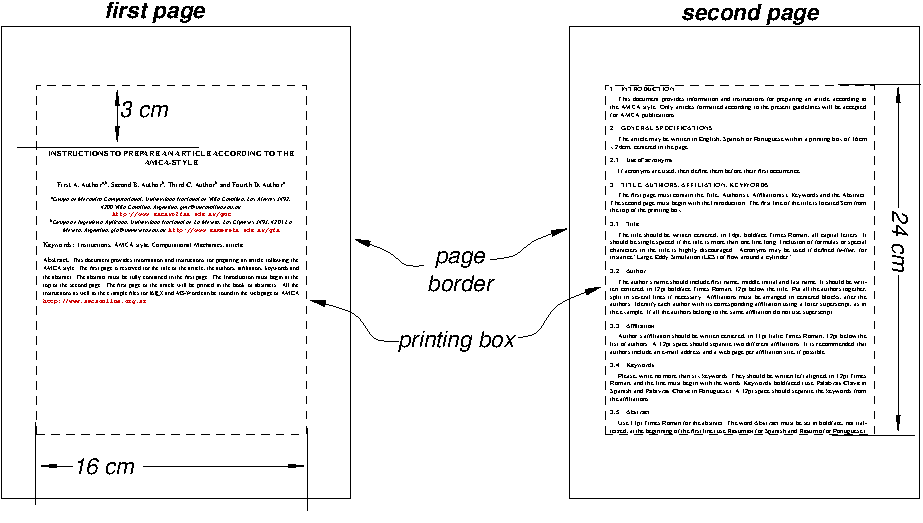
\includegraphics{firstpage}}
\caption{Page layout}
\label{fg:figure}
\end{figure*}

A 6pt space should separate the figure from the caption, and a
12pt space should separate the upper part of the figure and the
bottom of the caption from the surrounding text (see
Fig.~\ref{fg:figure}).

Figures should be referenced in the text. Color figures are welcomed.

\section{EQUATIONS}

A displayed equation is numbered, using Arabic numbers in parentheses.
It should be  centered, leaving a 6pt space above and below to separate it from
the surrounding text.

The following example is a simple single line
equation
%
\begin{equation}
Ax = b.
\end{equation}

The next example is a multi-line equation
%
\begin{equation} \label{eq:simple}  
\begin{aligned}
Ax& = b,\\
Ax& = c.
\end{aligned}
\end{equation}
%
If possible, internal PDF links must be generated for references to
equations. The recommended color for links to references in the text
is blue (e.g., see Eq.~(\ref{eq:simple})).

\section{TABLES}

All tables should be numbered consecutively and captioned, the caption
should be 10pt Times Roman, upper and lower case letters.

A space of 6pt separates the table from the caption, and 12pt space
separates the table from the surrounding text. For an example, see
Table~\ref{tab:n50}. Tables should be referenced in the text.

\begin{table}[htb]
\centering
\begin{tabular}{|c|c|c|c|}
\hline  & 20x20 mesh & 50x50 mesh & 100x100 mesh\\
\hline
\hline
 0 & 41.00 & 1.00 & 4.92\\
\hline
 1 & 40.86 & 1.02 & 4.88 \\
\hline
10 & 23.81 & 3.44 & 2.92 \\
\hline
50 & 5.62 & 64.20 & 1.08 \\
\hline
\end{tabular}
\caption{Condition number for the Stekhlov operator. }
\label{tab:n50}
\end{table}

\section{FORMAT OF REFERENCES}

References should be quoted in the text using the \emph{author-style}
(a.k.a. \emph{Harvard style}). References can be cited in
\emph{parenthetical} form \citep{zienkiewicz91,idelsohn94,meyer82,meyer82b}, or
in \emph{textual} form, e.g. see
\citet{zienkiewicz91,idelsohn94,meyer82,meyer82b}.  References are grouped
together and sorted alphabetically at the end of the article as shown
in these instructions. Do not include references that are not cited in
the article body. 

If possible, internal PDF links must be generated for citations. The
recommended color for links to references in the text is blue. The
preferred color for links to external references, as web pages, 
is red (e.g. \url{http://www.amcaonline.org.ar}).

\section{CONCLUSIONS}

Template files in TeX, \LaTeX{} and MS-Word may be found at the
AMCA web site: \url{http://www.amcaonline.org.ar}. 
Remember: {\bf Do not number the pages.}
%
\bibliography{eniefbib}
\end{document}
% $Id: amcapaper.tex,v 1.23 2006/08/14 16:58:45 mstorti Exp $
